\documentclass{article}
\author{Magnus Bergkvam}
\title{Project 1 \\ FYS-STK3155}
\usepackage{url}
\usepackage{amsmath}
\usepackage{graphicx}
\usepackage{subfig}
\graphicspath{{../figures/}}

% Julia code configuration
\usepackage[usenames,dvipsnames]{color} % more flexible names for syntax highlighting colors
\usepackage{listings}
\lstdefinelanguage{julia}
{
  keywordsprefix=\@,
  morekeywords={
    exit,whos,edit,load,is,isa,isequal,typeof,tuple,ntuple,uid,hash,finalizer,convert,promote,
    subtype,typemin,typemax,realmin,realmax,sizeof,eps,promote_type,method_exists,applicable,
    invoke,dlopen,dlsym,system,error,throw,assert,new,Inf,Nan,pi,im,begin,while,for,in,return,
    break,continue,macro,quote,let,if,elseif,else,try,catch,end,bitstype,ccall,do,using,module,
    import,export,importall,baremodule,immutable,local,global,const,Bool,Int,Int8,Int16,Int32,
    Int64,Uint,Uint8,Uint16,Uint32,Uint64,Float32,Float64,Complex64,Complex128,Any,Nothing,None,
    function,type,typealias,abstract
  },
  sensitive=true,
  morecomment=[l]{\#},
  morestring=[b]',
  morestring=[b]" 
}
\lstset{
basicstyle=\ttfamily, 
columns=fullflexible, % make sure to use fixed-width font, CM typewriter is NOT fixed width
numbers=left, 
numberstyle=\small\ttfamily\color{Gray},
stepnumber=1,              
numbersep=10pt, 
numberfirstline=true, 
numberblanklines=true, 
tabsize=4,
lineskip=-1.5pt,
extendedchars=true,
breaklines=true,        
keywordstyle=\color{Blue}\bfseries,
identifierstyle=, % using emph or index keywords
commentstyle=\sffamily\color{OliveGreen},
stringstyle=\color{Maroon},
showstringspaces=false,
showtabs=false,
upquote=false,
texcl=true % interpet comments as LaTeX
}
\lstset{
literate={σ}{{$\sigma$}}1
{λ}{{$\lambda$}}1
}
% End julia code

\begin{document}
\maketitle
\bibliographystyle{unsrt}

\section{Abstract}
We have in this project fitted various models on data generated from the
franke-function, a function which somewhat resembles a landscape, and real-world
geographical data. In both cases we have used polynomial features of
order 5 and fitted models to this franke-function both with and without added
noise.  The models we looked at was ridge, lasso and ordinary least squares.
For both the mean-squared-error and the $R^2$ score we saw that for the
franke-function without noise the ordinary least squares performed the best on
new data, but when we added noise-terms the lasso/ridge performed better.
Throughout the project we have clearly seen that less complex models often
perform better when we have some added noise (at least in the case when we have
somewhat limited data), but that this is not the case when there is no noise (or
a very high signal to noise-ratio). We have also explored how this result is
tied to the bias-variance tradeoff, and manifested the importance this has for
choosing the best model.

\section{Introduction}
Linear regression often is seen as a rather simple machine-learning method in
itself, but we do have less complex models than this again. Choosing the right
model complexity is well known as being an important part in getting the best
possible models for prediction, and in a lot of applications linear regression
offers just the right amount of complexity needed. Especially with cases where
our data is limited, or we have a low signal-to-noise ratio, linear regression
often performs very well \cite[p.~43]{hastie2009elements}. \\

However, when can it become beneficial to choose even less complex models than
this again? This is mainly what this project is about. We will mainly base this
project around the franke-function, which is a 2-dimensional function which
somewhat resembles a landscape \cite{franke2ddesc}. On the franke-function we
will fit ordinary least squares linear regression with polynomial features up to
order $5$ (with interactions), and then compare these results (using mainly the
mean squared error and $R^2$ metrics) to ridge and lasso regression on the
same data. We will also explore the performances of these models on some
real-world geographical data as well. For the franke-function we will be
generating two vectors of random points in $\left[ 0, 1 \right]$, and use
polynomial features with interactions of order $5$ for our data, for all our
models. We will also try to tie the results we get to the well-known
bias-variance tradeoff in machine learning, and on our way there explore various
resampling techniques for getting better estimates for model performances.
\\

We now get into a description of the models we have used, before we present the
results and finally conclude what we have found out.

\section{Methods}
\subsection{The franke function}
The franke-function is a function of two variables with the following definition:
\begin{align*}
    f(x,y) & = \frac{3}{4}\exp{\left(-\frac{(9x-2)^2}{4} - \frac{(9y-2)^2}{4}\right)}+\frac{3}{4}\exp{\left(-\frac{(9x+1)^2}{49}- \frac{(9y+1)}{10}\right)} \\
           & +\frac{1}{2}\exp{\left(-\frac{(9x-7)^2}{4} - \frac{(9y-3)^2}{4}\right)} -\frac{1}{5}\exp{\left(-(9x-4)^2 - (9y-7)^2\right) }
\end{align*}
We will use this function to generate a response from two explanatory variables
$x_1$ and $x_2$ both of which will be drawn randomly from $\left[ 0, 1 \right]$.
To get a visual picture of what the franke-function looks like on $\left[ 0, 1
        \right] \times \left[ 0, 1 \right]$ see figure \ref{franke-function-plot}.

\begin{figure}
    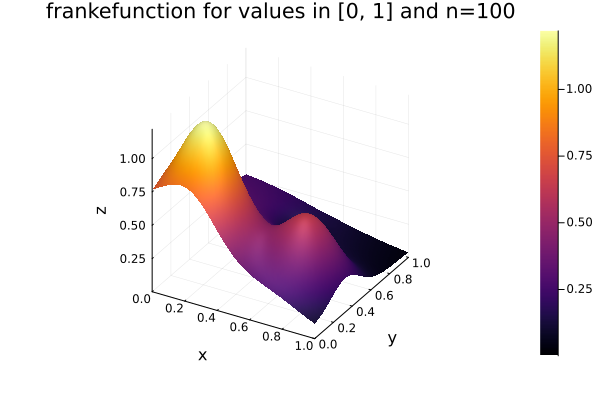
\includegraphics[scale=0.5]{frankefunction}
    \caption{A surface plot of the franke-function on $\left[ 0, 1 \right] \times \left[ 0, 1 \right]$}
    \label{franke-function-plot}
\end{figure}

Looking at such a plot we can see that the franke-function does somewhat
resemble a terrain. We will use the franke-function to generate data, both with
and without noise.  In the case without noise we will simply get the
following response:
$$\mathbf{y} = f(\mathbf{x_1}, \mathbf{x_2})$$
(Here where $f$ is applied element-wise to $\mathbf{x1}$ and $\mathbf{x2}$).
With noise we simply get:
$$\mathbf{y} = f(\mathbf{x1}, \mathbf{x2}) + \mathbf{\epsilon}$$
Where in this case $\epsilon_i \sim N(0, \sigma^2)$. We will use $\sigma = 0.1$
throughout all of our calculations (but this is easily adjustable in the code).

\subsection{Geographical data}
As mentioned, another source for data which was used for analysis of the
different models is some real-world geographical data. The data is stored as a
tiff image file and consists simply of a set of numerical values in a square
grid, where the numerical value indicates the height of the terrain in some way.
Figure \ref{landscape-plot} contains a plot of the data which we have used for
our analysis here.  The data is gathered from
\url{https://earthexplorer.usgs.gov/}, and we have here downloaded a region
around \textit{Møsvatn Austfjell} in Norway. This data includes a lot of
datapoints ($3601\times 1801 = 6485401$ to be exact), which is quite a lot more
than we need to fit a good model. Trying to fit a lot of different models to
such a big amount of data will often take a lot of memory and processing power,
so for this sake I have throughout our calculations limited the data to look at
only the first $400\times 500 = 20000$ observations, which should be more than
enough for our case. When reading the tiff-file we only get a matrix of values
out, but we will look at this as an image, and then use the position of the
response as explanatory variables for our model. In other words, if say the
fifth pixel in the fourth row has the value $10^{-5}$, the response will
obviously be $10^{-5}$, while the two explanatory variables will have values $5$
and $4$.  This way we will be able to gather data whose structure closely
resembles that of the franke-function. We will use thus us the same techniques
to setup design a matrix and response, as we did with the franke-function.

\begin{figure}
    \centerline{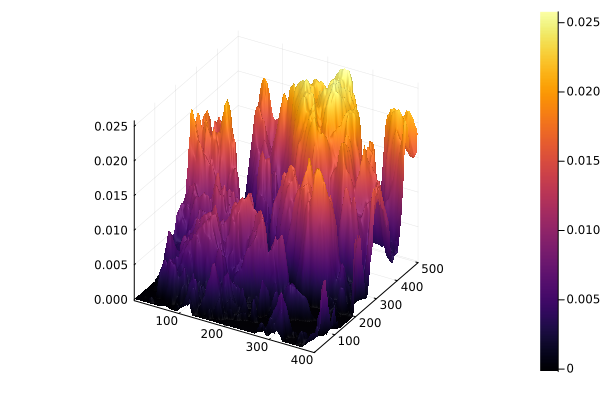
\includegraphics[scale=0.5]{landscapesurface}}
    \caption{A surface plot of the landscape data we have used. Keep in mind
        here that the axis here is simply the index of each datapoint in the
        tiff-file. This means that the axis here doesn't really tell us much, but
        shows the overall structure of the terrain nonetheless.}
    \label{landscape-plot}
\end{figure}

\subsection{Data/Data scaling}
The data and design matrix used throughout the project is mostly the same for
the different models, at least in the case of model evaluation for the
franke-function. The data we have used here is simply a collection of two
randomly generated datapoint-vectors $\mathbf{x}_1$ and $\mathbf{x}_2$, each of
size $200$, and the response is simply the value of the franke-function
evaluated at some point (plus some added noise in some cases). When we added
noise we have drawn this from the normal distribution with mean $0$ and
standard-deviance $0.1$ in order to not have too low of a signal-to-noise-ratio
(the franke-function gives quite low values). For the geographical data we load
the data in from a tiff file of geographical data, but the setup of the design
matrix is exactly the same, with the difference being that the $x1$'s $x2$'s and
response have been drawn directly from the tiff-file. The design matrix is
largely the same for the different models with some minor differences.  For the
$5$th order polynomials we have included in the first column the first-order
values of the $x$, the second column the second-order values of $x$, and so on.
The sixth to $10$ th column then is the first to fifth order terms of $y$ and
then we take $4 \cdot 4 = 16$ columns for interaction terms between the two
variables. A difference here is that for ordinary least squares we have added an
intercept by setting the first column to consist of only $1$.
\\
Throughout the whole of this project we have scaled the
features of the matrix, simply by centering the mean around $0$ and scaling by
the standard deviance. In the case of ordinary least squared regression this
scaling is not very important for model performance, as the model will be able
to scale the $\beta$'s correspondingly for different scaled data, but in the
case of ridge/lasso which both include a penalty term (see the ridge/lasso
sections), it becomes important to scale the data so that the scale of the data
doesn't affect how much we penalize the parameters (I will go into more detail
on this in the ridge/lasso sections).
\\
A last thing of note we have used throughout the project is train-test-splitting
(except when doing cross-validation). We then split our data into a train set
consisting of $80\%$ of the datapoints, and $20\%$ of the data for testing.
This lets us evaluate how well our model performs on "new" data, i.e. data the
model has not been trained on from the dataset. The reason this is important is
in order for us to recognize overfitted models, which often become the case when
we have a higher model complexity \cite[s.~7.2]{hastie2009elements}. In such
cases we could have a model that predicts the training data very well, but
generalizes very poorly to new data.  For the franke-function I have written a
function \textit{generatedata} which takes hand of all of the mentioned above
(here I am using Julia). It is a bit long, but well worth inclusion here as it
is central to all of the programs that use the franke-function:
\begin{lstlisting}[language=julia]
# Generate a design matrix consisting of random x-s (two explanatory variables)
# with a polynomial of a given order (we will use order 5 for our analysis
# mainly). Additionally includes options for adding intercept column, noise,
# number of observations and random seed.
function generatedata(order::Int64; split=true, include_intercept=false, add_noise=false, noise_σ=0.1, n=200, custom_seed=1000)
    # Setting the seed for train test splitting and random x1/x2
    seed!(custom_seed)

    # Generating x-s
    x1 = rand(n)
    x2 = rand(n)

    # Creating the design matrix
    X = generatedesignmatrix(x1, x2, order)

    # Creating the response
    y = Functions.frankefunction(x1, x2)


    # Shuffle before train-test splitting
    Xs, ys = shufflematrices(X, y)

    # Train-test splitting
    if !split
        return standardscale(Xs, Xs), ys
    end
    indextosplitat = convert(Int, floor(size(Xs, 1) * 0.8))
    X_train, X_test = Xs[1:indextosplitat, :], Xs[(indextosplitat+1):size(Xs, 1), :]
    y_train, y_test = ys[1:indextosplitat, :], ys[(indextosplitat+1):size(ys, 1), :]

    # Scaling X\_train/X\_test
    # Here we create a copy of the X\_train matrix as we want to use the
    # column-means of this to scale both the X\_train and X\_test columns.
    X_train_original = copy(X_train)
    X_train = standardscale(X_train, X_train_original)
    # We use the column means from the original X\_train to subtract from the
    # columns in X\_test.
    X_test = standardscale(X_test, X_train_original)

    if add_noise
        # Add response with noise
        y_train += rand(Normal(0, noise_σ), length(y_train))
        y_test += rand(Normal(0, noise_σ), length(y_test))
    end

    if include_intercept
        X_train = [ones(size(X_train, 1)) X_train]
        X_test = [ones(size(X_test, 1)) X_test]
    end

    return X_train, X_test, y_train, y_test
end
\end{lstlisting}

Here we have used some other local functions like standardscale (scaling as
described in the scaling section in this report) and shufflematrices (random
shuffles rows in a matrix), which it should be clear what these do based on
their name, but I'll also include the implementation of the
\textit{generatedesignmatrix}, as it is very central for all the calculations we
have done:
\begin{lstlisting}[language=julia]
# Generate a matrix with features as polynomial terms with interactions
function generatedesignmatrix(x1, x2, order)
    X = zeros((length(x1), 2 * order + (order - 1)^2))
    for i in 1:order
        X[:, i] = x1 .^ i
        X[:, order+i] = x2 .^ i
    end
    for i in 1:(order-1)
        for j in 1:(order-1)
            X[:, 1+order+i*(order-1)+j] = (x1 .^ i) .* (x2 .^ j)
        end
    end

    return X
end
\end{lstlisting}

Shuffling the data is perhaps not nessecary here in the case of the
franke-function seeing as the explanatory variables are randomly drawn (but I
have done so anyway just out of good practice), however in the case of the
landscape data this is very important, as here the data is sorted when reading
the data in, and if we then do not shuffle the data before, and we then apply
train-test-splitting, we will get different regions of our response for the
training and testing data, in other words, the model will be trained on data
from some area and tested on data from another area, which will then probably
give quite poor performance (unless the two regions the train-data and test-data
are gathered from are very similar).


\subsection{Ordinary least squares}
The first, and conceptually simplest, model we looked at in this project was the
ordinary least squares linear regression. Before we further describe this
method, denote $\mathbf{X}$ as our design-matrix. This is generated as described
already, by using polynomial features up to order $5$. However unlike for the
other models, our design matrix in this case will have the first column just
consisting of $1$s. This is to add an intercept-term.  Ordinary least squares
regression finds the $\mathbf{\beta}$ which minimizes the loss-function (this
optimal value we call $\hat{\mathbf{\beta}}$) given like:
$$C(\beta) = (y - X\mathbf{\beta})^T (y - X\mathbf{\beta})$$
Then to find the $\hat{\beta}_{ols} = (X^T_{train} X_{train})^{-1} X^T_{train}
    y_{train}$. We then can make predictions for the training-set by:
$$\hat{y}_{train} = X_{train} \hat{\beta}_{ols}$$
and for the traning set:
$$\hat{y}_{test} = X_{test} \hat{\beta}_{ols}$$

\subsection{Ridge and lasso}
Ridge and lasso is in lots of ways very similar to ordinary least squares
regression. The setup of the model is exactly the same, where for both these
models we estimate some parameter vector $\mathbf{\beta}$, where we assume
$$\mathbf{y} = \mathbf{X} \mathbf{\beta} + \mathbf{\epsilon}$$
The difference arises with the cost function we minimize to estimate the parameters. For ridge we use:
$$C(\mathbf{\beta}) = \left(\sum_{i=1}^{n} (y_i - \beta_0 - \beta_1 x_{i 1} - \dots - \beta_{p} x_{i p})\right) + \lambda \sum_{i=1}^p \beta_i^2$$
and for lasso:
$$C(\mathbf{\beta}) = \left(\sum_{i=1}^{n} (y_i - \beta_0 - \beta_1 x_{i 1} - \dots - \beta_{p} x_{i p})\right) + \lambda \sum_{i=1}^p \lvert \beta_i \rvert$$
for some hyperparameter $\lambda$, which determines how much we want to penalize
high parameter values. Keep in mind that we do not here penalize the intercept
in the loss-function. We often do this because we in general are ok with a
somewhat high intercept, because this often lead to better performance. We will
therefore when writing our code, fit ridge regression without a intercept (by
not including a first column of only $1$s), and then based on the other
parameters calculate the optimal intercept $\beta_0$ which leads to the optimal
loss. This we can do by the following equation:
$$\beta_0 = \frac{1}{n} \sum_{i=0}^{n-1} y_i - \frac{1}{n} \sum_{i=0}^{n-1} \sum_{j=1}^{p-1} X_{i j} \beta_j$$
As proved in \cite[s.~Further manipulations]{week35notes}.
(To get our estimate we simply replace our $\beta_i$s with their estimates).
Furthermore, from the cost-function we see further why it is important to scale
the data beforehand. If we have data with widely different scaling this will
impact how the optimal corresponding $\beta$ to the feature should be (not
regarding the penalty term). If we have a feature with very high values, this
$\beta$ will be smaller, than if we use a smaller scale/unit. But then this term
$\beta^2$ will be much bigger, and we will reduce the cost much further by
decreasing this parameter than if it had a smaller scale. In order to hinder
this happening it them becomes important to scale the features somewhat alike,
so that the scale the features is given on does not determine the fit we get.

\subsection{The bias variance tradeoff}
Central in this project will be the bias variance tradeoff. This is the reason
why ridge and lasso often can give better predictions than ordinary least
squares. We will here derive the bias-variance equation. Consider the model
$\mathbf{y} = f(\mathbf{x}) + \epsilon$ where $E(\epsilon) = 0$ and
$Var(\epsilon) = \sigma^2$, for some function $f$. The job in machine-learning
is to estimate this $f$. We call $\hat{f}$ some estimate of this function $f$.
We then get $\hat{\mathbf{y}} = \hat{f}(\mathbf{x})$, which is some prediction.
We consider the squared error of one such prediction $(y_i - \hat{y}_i)^2$. We
now want to find an expression for this mean-squared error, however this is a
little difficult to calculate as both terms here are stochastic. We therefore
calculate the expectance of this expression, in which we get:
\begin{align*}
    E((y - \hat{y})^2) & = E((f(x) + \epsilon - \hat{f}(x))^2)                                                      \\
                       & = E((\epsilon + (f(x) - \hat{f}(x)))^2)                                                    \\
                       & = E(\epsilon^2 + 2\cdot \epsilon \cdot (f(x) - \hat{f}(x)) + (f(x) - \hat{f}(x))^2)        \\
                       & = E(\epsilon^2) + 2\cdot E(\epsilon) \cdot E(f(x) - \hat{f}(x)) + E((f(x) - \hat{f}(x))^2) \\
                       & = E((\epsilon - E(\epsilon))^2) + E((f(x) - \hat{f}(x))^2)                                 \\
                       & = \sigma^2 + E((f(x) - \hat{f}(x))^2)                                                      \\
\end{align*}
Here we have used independence of $\epsilon$ from $f(x) - \hat{f}(x)$ which
stems from the fact that we may assume that $\hat{f}(x)$ and $\epsilon$ are
independent. We now focus on calculating the second part of this, i.e. $E((f(x)
    - \hat{f}(x))^2)$. We have:
\begin{align*}
     & E\left[(f(\mathbf{x}) - \hat{f}(\mathbf{x}))^2\right]                                                                                                                                                                                             \\
     & = E\left[((f(\mathbf{x}) - E(\hat{f}(\mathbf{x}))) + (E(\hat{f}(\mathbf{x})) - \hat{f}(\mathbf{x})))^2\right]                                                                                                                                     \\
     & = E\left[(f(\mathbf{x}) - E(\hat{f}(\mathbf{x})))^2 + 2\cdot (f(\mathbf{x}) - E(\hat{f}(\mathbf{x}))) \cdot (E(\hat{f}(\mathbf{x})) - \hat{f}(\mathbf{x})) + (E(\hat{f}(\mathbf{x})) - \hat{f}(\mathbf{x}))^2\right]                              \\
     & = E\left[(f(\mathbf{x}) - E(\hat{f}(\mathbf{x})))^2\right] + 2\cdot E\left[(f(\mathbf{x}) - E(\hat{f}(\mathbf{x}))) \cdot (E(\hat{f}(\mathbf{x})) - \hat{f}(\mathbf{x}))\right] + E\left[(E(\hat{f}(\mathbf{x})) - \hat{f}(\mathbf{x}))^2 \right] \\
     & = (f(\mathbf{x}) - E(\hat{f}(\mathbf{x})))^2 + 2\cdot E\left[(f(\mathbf{x}) - E(\hat{f}(\mathbf{x})))\right] \cdot E\left[(E(\hat{f}(\mathbf{x})) - \hat{f}(\mathbf{x}))\right] + E\left[(E(\hat{f}(\mathbf{x})) - \hat{f}(\mathbf{x}))^2 \right] \\
     & = (f(\mathbf{x}) - E(\hat{f}(\mathbf{x})))^2 + 2\cdot E\left[(f(\mathbf{x}) - E(\hat{f}(\mathbf{x})))\right] \cdot (E(\hat{f}(\mathbf{x})) - E(\hat{f}(\mathbf{x}))) + E\left[(E(\hat{f}(\mathbf{x})) - \hat{f}(\mathbf{x}))^2 \right]            \\
     & = (E(\hat{f}(\mathbf{x})) - f(\mathbf{x}))^2 + E\left[(\hat{f}(\mathbf{x}) - E(\hat{f}(\mathbf{x})))^2 \right]                                                                                                                                    \\
\end{align*}
Typically in machine learning we call the first term here the squared bias of the
model, and the second term the variance. In total we get:
$$E((y - \hat{y})^2) = \sigma^2 + (E(\hat{f}(\mathbf{x})) - \hat{f}(\mathbf{x}))^2 + E\left[(\hat{f}(\mathbf{x}) - E(\hat{f}(\mathbf{x})))^2\right] = \sigma^2 + Bias(\hat{f}(x))^2 + Var(\hat{f}(x))$$
We see that the expected squared prediction error is given as a sum of the
variance of the noise $\sigma^2$, the bias of our model, and the variance of our
model. Here $\sigma^2$ is an irreducible part we cannot control by the choice of
our model, while the bias and variance is dependent on the type of model that we
use \cite[s.~2.9]{hastie2009elements}. We can see here that the bias is the
difference between our models' expectation and the actual expectation $f(x)$.
The variance is how much the model varies for the different training data (try to rewrite this). We
now go more into detail of this for the models
we use in the project.

\subsection{Bias and variance of ols/ridge/lasso}
Instrumental to explaining the bias and variance of the different models, we
will calculate bias and variance for the parameters in ols and ridge regression.
In the case of ordinary least squares we assume:
$$y_i = \mathbf{X}_{i *} \mathbf{\beta} + \epsilon_i$$
With $\epsilon_i \sim N(0, \sigma^2)$. Looking at the expectance of $y_i$ it is
easy then to see:
\begin{align*}
    E(y_i) & = E\left[ \mathbf{X}_{i *} \mathbf{\beta} + \epsilon_i \right]                 \\
           & = E\left[ \mathbf{X}_{i *} \mathbf{\beta} \right] + E\left[ \epsilon_i \right] \\
           & = \mathbf{X}_{i *} \mathbf{\beta} + 0                                          \\
           & = \mathbf{X}_{i *}\mathbf{\beta}
\end{align*}
(Here we have used the fact that $\mathbf{X}_{i *} \mathbf{\beta}$ is
non-stochastic and $E(\epsilon_i) = 0$). Calculating the variance of $y_i$ we
have:
\begin{align*}
    Var(y_i) & = Var(\mathbf{X}_{i, *} \mathbf{\beta} + \epsilon_i) \\
             & = Var(\epsilon_i)                                    \\
             & = \sigma^2
\end{align*}
(Again we have here used that $\mathbf{X}_{i *} \mathbf{\beta}$ is non-stochastic).
This is enough to conclude that $y_i \sim N(\mathbf{X}_{i *} \mathbf{\beta},
    \sigma^2)$.  To analyze our $\mathbf{\hat{\beta}}$ we can look at the
expectance/variance of this. In order to elegantly calculate this we use two
somewhat basic results, which I have proved in the appendix. Let $\mathbf{A}$ be a
non-stochastic ($p\times n$) matrix and $\mathbf{X}$ be a stochastic ($n \times
    p$) vector. We then have the following two results.
$$E(\mathbf{A} \mathbf{X}) = \mathbf{A} E(\mathbf{X})$$
and
$$Var(\mathbf{A} \mathbf{X}) = \mathbf{A} Var(\mathbf{X}) \mathbf{A}^T$$
Using these results and using that $\hat{\beta} = (\mathbf{X}^T \mathbf{X})^{-1} \mathbf{X}^T \mathbf{Y}$:
\begin{align*}
    E(\mathbf{\hat{\beta}}) & = E((\mathbf{X}^T \mathbf{X})^{-1} \mathbf{X}^T \mathbf{Y})             \\
                            & = (\mathbf{X}^T \mathbf{X})^{-1} \mathbf{X}^T E(\mathbf{Y})             \\
                            & = (\mathbf{X}^T \mathbf{X})^{-1} \mathbf{X}^T \mathbf{X} \mathbf{\beta} \\
                            & = \mathbf{\beta}
\end{align*}
and
\begin{align*}
    Var(\mathbf{\hat{\beta}}) & = Var((\mathbf{X}^T \mathbf{X})^{-1} \mathbf{X}^T \mathbf{Y})                                                              \\
                              & = (\mathbf{X}^T \mathbf{X})^{-1} \mathbf{X}^T Var(\mathbf{Y}) \left( (\mathbf{X}^T \mathbf{X})^{-1} \mathbf{X}^T \right)^T \\
                              & = (\mathbf{X}^T \mathbf{X})^{-1} \mathbf{X}^T \sigma^2 I \mathbf{X} \left( (\mathbf{X}^T \mathbf{X})^{-1} \right)^T        \\
                              & = \sigma^2 (\mathbf{X}^T \mathbf{X})^{-1} \mathbf{X}^T \mathbf{X} \left((\mathbf{X}^T \mathbf{X})^T \right)^{-1}           \\
                              & = \sigma^2 (\mathbf{X}^T \mathbf{X})^{-1} \mathbf{X}^T \mathbf{X} (\mathbf{X}^T \mathbf{X})^{-1}                           \\
                              & = \sigma^2 (\mathbf{X}^T \mathbf{X})^{-1}
\end{align*}
For ridge we have that $\hat{\beta}_{ridge} = (\mathbf{X}^T \mathbf{X} + \lambda
    \mathbf{I}_{p p})^{-1} \mathbf{X}^T \mathbf{Y}$. We now calculate the expectance
of this:
\begin{align*}
    E(\mathbf{\hat{\beta}}_{ridge}) & = E((\mathbf{X}^T \mathbf{X} + \lambda \mathbf{I}_{p p})^{-1} \mathbf{X}^T \mathbf{Y})             \\
                                    & = (\mathbf{X}^T \mathbf{X} + \lambda \mathbf{I}_{p p})^{-1} \mathbf{X}^T E(\mathbf{Y})             \\
                                    & = (\mathbf{X}^T \mathbf{X} + \lambda \mathbf{I}_{p p})^{-1} \mathbf{X}^T \mathbf{X} \mathbf{\beta}
\end{align*}
and for the variance:
\begin{align*}
    Var(\mathbf{\hat{\beta}}_{ridge}) & = Var((\mathbf{X}^T \mathbf{X} + \lambda \mathbf{I}_{p p})^{-1} \mathbf{X}^T \mathbf{Y})                                                                                \\
                                      & = (\mathbf{X}^T \mathbf{X} + \lambda \mathbf{I}_{p p})^{-1} \mathbf{X}^T Var(\mathbf{Y})  ((\mathbf{X}^T \mathbf{X} + \lambda \mathbf{I}_{p p})^{-1} \mathbf{X}^T)^T    \\
                                      & = (\mathbf{X}^T \mathbf{X} + \lambda \mathbf{I}_{p p})^{-1} \mathbf{X}^T \sigma^2 \mathbf{I}_{p p} \mathbf{X} (\mathbf{X}^T \mathbf{X} + \lambda \mathbf{I}_{p p})^{-1} \\
                                      & = \sigma^2 (\mathbf{X}^T \mathbf{X} + \lambda \mathbf{I}_{p p})^{-1} \mathbf{X}^T \mathbf{X} ((\mathbf{X}^T \mathbf{X} + \lambda \mathbf{I}_{p p})^{-1})^T              \\
\end{align*}
Using these results it is easy to see that under the assumption that $\mathbf{y}
    = \mathbf{X}\mathbf{\beta} + \mathbf{\epsilon}$, that the ordinary least squares
model is unbiased, while this is not the case for ridge-regression. However we
see that the variance of the ridge-model has considerably lower variance than
the ols. This does allow for ridge to outperform ols, since the bias-variance
tradeoff states that the expected prediction error is the sum of the bias and
variance. Much of this effect also applies for lasso regression as well as this
also has a higher bias and lower variance than ols.

\subsection{Bootstrap}
Since this project essentially boils down to comparing metrics for different
models on some data it becomes important that these metrics which we calculate
are reliable. In the case of the franke-function we have used $200$ datapoints,
which we have split into a training-set and test-set. We have then trained the
data on the training-set and then evaluated the trained model on the test-set,
however since the test-set is only $20\%$ of our datapoints, we have that this
test-set is rather small. This can make the test-error which we achieve quite
specific to the model which we have trained, and our metrics may not be that
reliable. In order to combat this we will use resampling techniques. One way
which do this by is using bootstrap. We will use bootstrapping to estimate the
MSE and R\^2 scores on the test-data. Thus we will first have to split the data
into a training and testing-set like before. Then we draw bootstrap samples
(i.e. we draw $n$ observations from the $n\times p$ design-matrix $X_{train}$
with replacement) from the training-data and fit the model on this data and
evaluate the metrics on the test-data. We do this $B$ times and take the mean of
these metrics to get our final estimates. This often will give us a better
estimate for the metrics because it does not require assumptions on error terms,
which causes bootstrap to give us more reliable results when we have a smaller
sample size (which we do in this case, especially for) \cite[s.~5.3]{lecturenotes5}.

\subsection{Cross-validation}
K-fold cross-validation is another resampling-technique which also can better our
estimates for the various metrics. Unlike with bootstrapping we don't need to
split the data into a training-set or test-set anymore. K-fold cross-validation
works by splitting the data into $K$ folds of as equal sizes as possible. Now
denote for some $1 \leq i \leq K$ $X^{-i}$ as the design-matrix with fold $i$
excluded, and $X^i$ as the data for fold $i$ of our design-matrix. For
cross-validation we do for $i = 1, \dots, K$:
\begin{enumerate}
    \item Fit our model on $X^{-i}$
    \item Evaluate our metric on $X^{i}$
\end{enumerate}
We then, much like bootstrapping average over all the metrics to get our final
metric. The reason this improves the estimate for the metrics is that since
every fold is used for evaluating the metric, that every observation also is
used in the estimate for our final metric. This is in contrast to our earlier
estimate, which the metric is only evaluated using the rather small test-set.
This should give us a better estimate for the true MSE or R\^2.
\section{Results}
\subsubsection{Franke-function}
\subsubsection{Ordinary least squares}
We have located the code for performing ordinary least squares regression on the
franke-function with polynomial features up to order $5$ in the
\textbf{LinearRegression.jl} on the project repository
\cite{githubrepoproject1}. Running this we can extract the following metrics:\\
\begin{tabular}{| c | c | c | c | c |}
          & \multicolumn{2}{|c|}{Without noise} & \multicolumn{2}{|c|}{With noise}                           \\
          & MSE                                 & R\^2                             & MSE        & R\^2       \\
    TRAIN & $0.001046$                          & $0.985926$                       & $0.008400$ & $0.905406$ \\
    TEST  & $0.007677$                          & $0.907600$                       & $0.058654$ & $0.395051$ \\
\end{tabular}

We see there is quite good performance on the training-set and test-set when
noise is not included. When we include noise-terms the model-performance on the
training data is still quite good, but with the test-data we get rather poor
results.

\subsubsection{Ridge}
If we run the \textbf{Ridge.jl} program in the project repository
\cite{githubrepoproject1}, we can extract the following results:\\
\begin{tabular}{| c | c | c | c | c |}
          & \multicolumn{2}{|c|}{Without noise} & \multicolumn{2}{|c|}{With noise}                           \\
          & MSE                                 & R\^2                             & MSE        & R\^2       \\
    TRAIN & $0.001046$                          & $0.985926$                       & $0.008400$ & $0.905406$ \\
    TEST  & $0.003592$                          & $0.956765$                       & $0.017352$ & $0.821028$ \\
\end{tabular}

With the optimal $\lambda$ for test-data without noise being $1.659587\cdot
    10^{-2}$ and when we include noise it becomes $1.513561$.
Additionally we can see how the MSE and R\^2 score varies with different values
of the hyperparameter $\lambda$ with the following two plots:\\

\begin{figure}
    \centerline{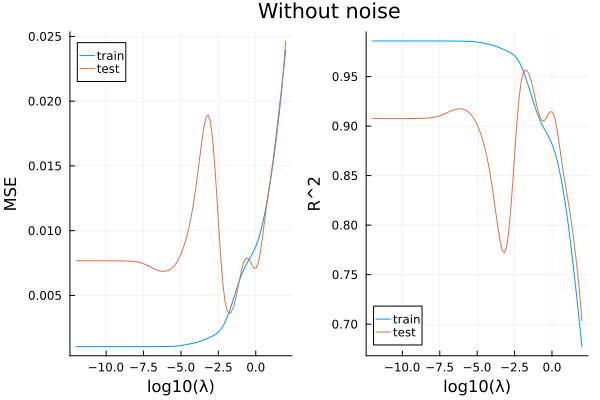
\includegraphics[scale=0.5]{ridge_without_noise}}
    \caption{A plot of the $\lambda$ in a ridge-model without noise on log10-scale plotted against the MSE and R\^2. We see that performances of these metrics goes a bit up and down for the different values of $\lambda$.}
    \label{Ridge-with-noise}
\end{figure}

\begin{figure}
    \centerline{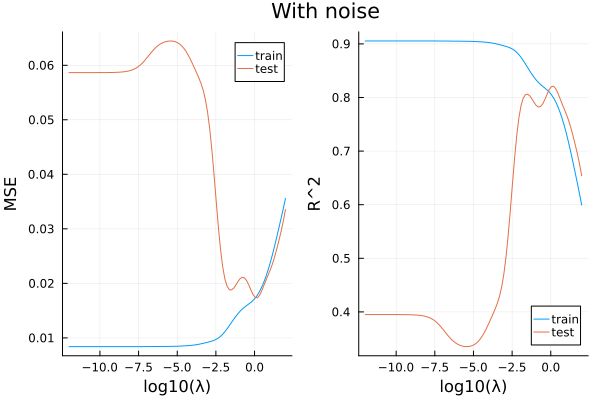
\includegraphics[scale=0.5]{ridge_with_noise}}
    \caption{A plot of the $\lambda$ in a ridge-model with $\lambda$s on log10-scale plotted against the MSE and R\^2. We see a somewhat similar relationship as for the case with noise, but with greater scales on the y-axis}
    \label{Ridge-no-noise}
\end{figure}

\subsubsection{Lasso}
The \textbf{Lasso.jl} on the project repo \cite{githubrepoproject1} runs lasso
regression on the franke-function data and calculates the MSE and R\^2. Running
this we get:

\begin{tabular}{| c | c | c | c | c |}
          & \multicolumn{2}{|c|}{Without noise} & \multicolumn{2}{|c|}{With noise}                           \\
          & MSE                                 & R\^2                             & MSE        & R\^2       \\
    TRAIN & $0.003280$                          & $0.955866$                       & $0.011319$ & $0.872539$ \\
    TEST  & $0.002737$                          & $0.967054$                       & $0.016451$ & $0.830329$ \\
\end{tabular}

\begin{figure}
    \centerline{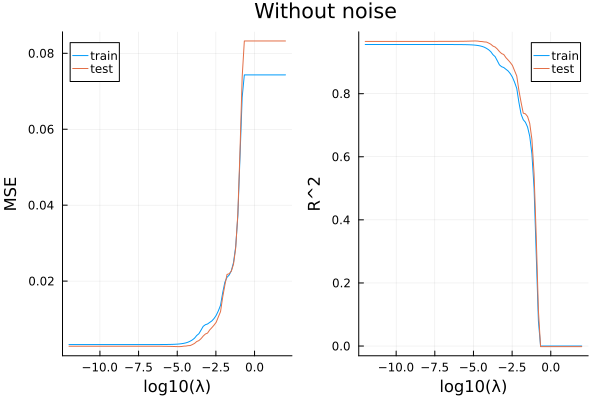
\includegraphics[scale=0.5]{lasso_without_noise}}
    \caption{A plot of the $\lambda$ in a lasso-model with $\lambda$s on log10-scale plotted against the MSE and R\^2. Unlike the Ridge-case this completely flattens out at the end. This is due to the fact that for such high values of $\lambda$ the model-parameters which minimize the loss is simply with all the $\beta$s (other than the intercept term) is $0$}
    \label{Lasso-no-noise}
\end{figure}
\begin{figure}
    \centerline{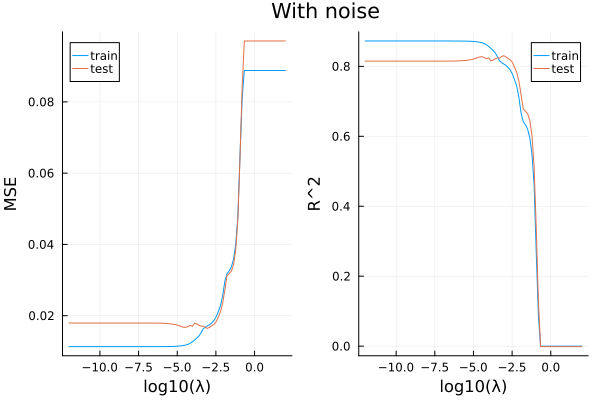
\includegraphics[scale=0.5]{lasso_with_noise}}
    \caption{A plot of the $\lambda$ in a lasso-model with $\lambda$s on log10-scale plotted against the MSE and R\^2. We see the same flattening as in figure \ref{Lasso-no-noise}}
    \label{Lasso-with-noise}
\end{figure}

\subsubsection{Performance with more complex models}
Up until now we have used only polynomial features of order 5. The
\textbf{Resampling.jl} and \textbf{ResamplingCV.jl} explores fitting the
franke-function to data with more polynomial degrees, with the metrics
calculated using bootstrap and cross-validation respectively. Running these
programs we gather some plots of the mean squared errors plotted against the
model complexity, this time in the form of orders of polynomial features. Figure
\ref{bootstrap-bias-var} shows the mse using ols, calculated using
bootstrapping, while figure \ref{crossval-ols}, \ref{crossval-ridge} and
\ref{crossval-lasso} show the same graphs for ols, ridge and lasso respectively,
these calculated using cross-validation.

\begin{figure}
    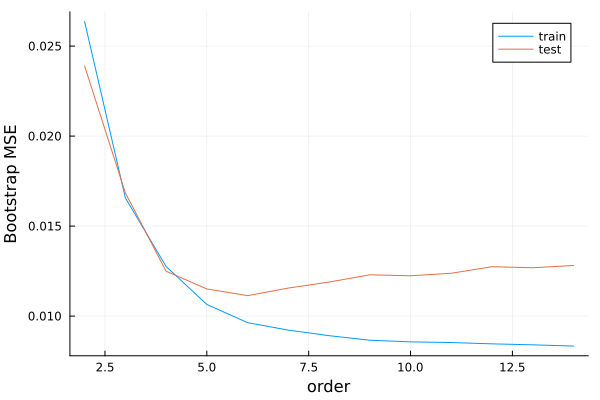
\includegraphics[scale=0.5]{bootstrapbiasvariance}
    \caption{The MSE calculated using bootstrap plotted against the increasing
        orders of polynomial features. For the training we unsurprisingly get a
        lower and lower MSE as we increase the orders of polynomials, but for the
        testing data we get at first a lower MSE by increasing the polynomials up
        until about order $6$ where it after this increases. This is to be expected
        from what we know of the bias-variance tradeoff}
    \label{bootstrap-bias-var}
\end{figure}

\begin{figure}
    \centering
    \subfloat{{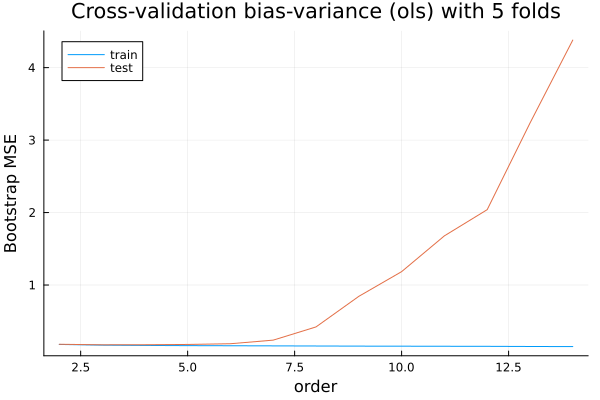
\includegraphics[width=5.5cm]{crossvalbiasvariance_ols__5_folds}}}
    \quad
    \subfloat{{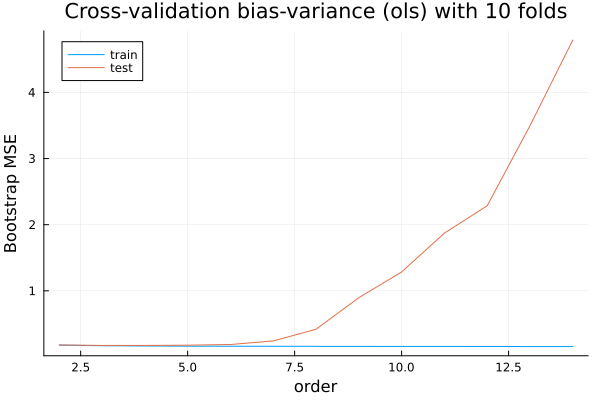
\includegraphics[width=5.5cm]{crossvalbiasvariance_ols__10_folds}}}
    \caption{Side by side cross-validated estimates of the mean squared error of
        ordinary least squares models with varying orders of features with $k=5$ and
        $k=10$ folds. We see that the mean squared error for the test data rapidly
        increases after polynomial order $\approx 6$. Since both of the results for
        $k=5$ and $k=10$ seem to be very similar we can be confident that we do not
        need to increase the amount of folds here to get a more reliable result
        - the result has already converged.}
    \label{crossval-ols}
\end{figure}
\begin{figure}
    \centering
    \subfloat{{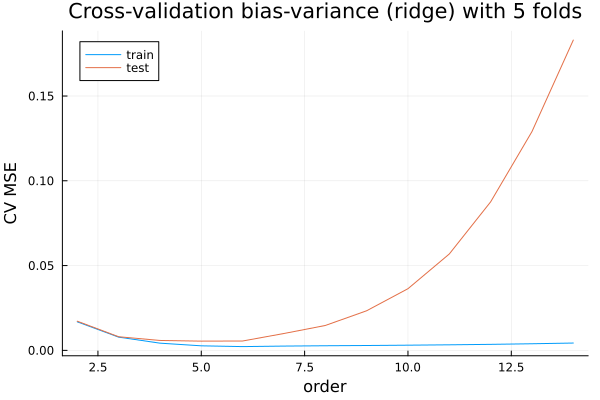
\includegraphics[width=5.5cm]{crossvalbiasvariance_ridge__5_folds}}}
    \quad
    \subfloat{{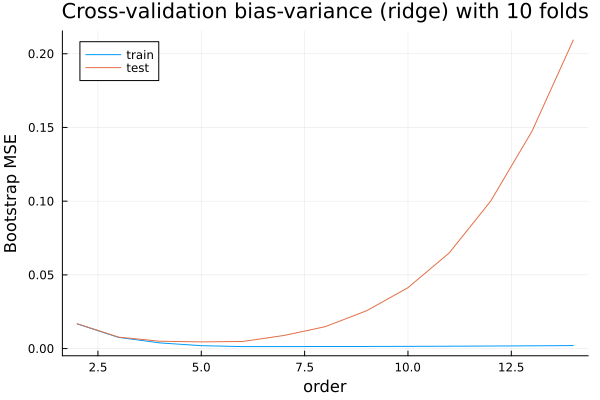
\includegraphics[width=5.5cm]{crossvalbiasvariance_ridge__10_folds}}}
    \caption{Side by side cross-validated estimates of the mse, this time for
        ridge models with varying degrees of polynomial features and $k=5$ and
        $k=10$ this time as well. We get again very similar results for the two
        sizes of folds. Here we see clearer that the test MSE decreases at first as
        we get higher order polynomial features, before it increases again as we get
        more and more complex models. We also notice that the scale here is much
        smaller than in the ols case, likely due to ridge being a less complex
        model.}
    \label{crossval-ridge}
\end{figure}

\begin{figure}
    \centering
    \subfloat{{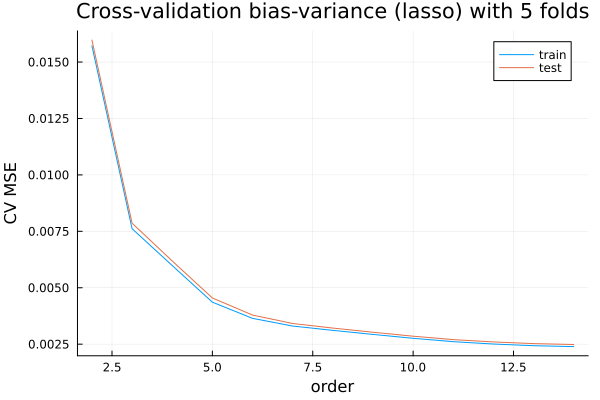
\includegraphics[width=5.5cm]{crossvalbiasvariance_lasso__5_folds}}}
    \quad
    \subfloat{{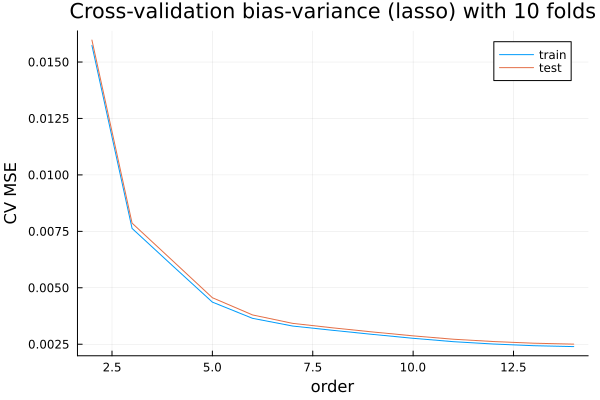
\includegraphics[width=5.5cm]{crossvalbiasvariance_lasso__10_folds}}}
    \caption{Side by side cross-validated estimates of the mse, finally this time for lasso models with varying degrees of polynomial features and $k=5$ and
        $k=10$ folds this time as well, with the same result for the two
        different fold sizes. Interesting here is that we actually get better
        and better performance as we increase the polynomial order it could look
        like. Keep in mind though that we only have tested up to order $14$. If
        we were to increase this even more, we likely would get problems so long
        as the $\lambda$ parameter stays the same.}
    \label{crossval-lasso}
\end{figure}

\subsection{Landscape data}


\section{Analysis}
As we can see from the results, the ordinary least squares performs rather good
on the models without noise, with ordinary least squares regression performing
considerably better than both ridge and lasso, with ridge and lasso having quite
comparable results. Looking at

\section{Conclusion}

\section{Appendix}

\subsection{Project code (github)}
All the julia programs described in the report and with the full source code can be
found at:
\url{https://github.com/magnouvean/ml-physics-projects/tree/main/project1/julia}

\subsection{Expectance and variance with matrices}
Let $A$ be a non-stochastic matrix and $\mathbf{X}$ be a stochastic vector. We have:
$$E(A \mathbf{X}) = (E(A \mathbf{X})_1, \dots, E((A \mathbf{X})_n))^T$$
We have:
$$E(A \mathbf{X})_i = E((A \mathbf{X})) = E(A_{i *} \mathbf{X}) = A_{i *} E(\mathbf{X})$$
Hence we see that $E(A \mathbf{X}) = A E(\mathbf{X})$.
Note also that from this it follows that $E(A \mathbf{X})^T = (A
    E(\mathbf{X}))^T = E(\mathbf{X})^T A^T$ (we will use this for calculating the
variance expression).
Additionally we have for $E(X A^T)$:
$E(X A^T)_i = E((X A^T)_i) = E(X_i )$

We now want to look at the case of the variance. We have:
\begin{align*}
    Var(A \mathbf{X}) & = E((A \mathbf{X} - E(A \mathbf{X})) (A \mathbf{X} - E(A \mathbf{X}))^T)                                                                       \\
                      & = E((A \mathbf{X})(A \mathbf{X})^T  - A \mathbf{X} E(A \mathbf{X})^T - E(A \mathbf{X}) (A \mathbf{X})^T + E(A \mathbf{X}) E(A \mathbf{X})^T)   \\
                      & = E(A \mathbf{X}\mathbf{X}^T A^T  - A \mathbf{X} E(\mathbf{X})^T A^T - A E(\mathbf{X}) \mathbf{X}^T A^T + A E(\mathbf{X}) E(\mathbf{X})^T A^T) \\
                      & = E(A (\mathbf{X}\mathbf{X}^T  - \mathbf{X} E(\mathbf{X})^T - E(\mathbf{X}) \mathbf{X}^T + E(\mathbf{X}) E(\mathbf{X})^T ) A^T)                \\
                      & = A E(A (\mathbf{X} - E(\mathbf{X})) (\mathbf{X} - E(\mathbf{X}))^T) A^T                                                                       \\
                      & = A Var(\mathbf{X}) A^T                                                                                                                        \\
\end{align*}


\bibliography{./sources.bib}

\end{document}